\section{Experiments and Results}\label{sec:experiments}
Experiments were performed on both stationary and moving datasets.  Our \texttt{stationary} dataset is approximately 22 minutes long and was collected using the Upson Hall antenna on November 11, 2013 starting at approximately 7:39 PM EST.  Weather parameters for the neutral atmosphere corrections were obtained from wunderground.com.  Our moving datasets include those distributed on the course website.  While we evaluated our methods on all datasets, we present in this paper results for \texttt{airportloop} and \texttt{cudtrt13triphammercu}. \texttt{airportloop} offers an interesting case where most of the route is unaffected by multipath errors since tall buildings are not present.  Additionally, the weather measurements should be quite accurate, assuming they were acquired using the weather station located at the airport.  In contrast, \texttt{cudtrt13triphammercu} offers many challenging examples of line-of-sight occlusion and multipath reflections as well as long stretches of highway for the filter to recover.

We evaluate several versions of our time-varying Kalman filters, each with different turning parameters.  In addition, we also compare to results obtained by using a steady-state Kalman filter built with MATLAB's \texttt{dlqe}, and the two static filters described in~\cite{course}.  Interactive, qualitative results for all datasets can be viewed at \url{http://mae5150.kmatzen.com} until February 2014.  Many of the static filter and steady-state Kalman filter results are omitted from this paper since they largely overlap and are hard to visualize.

Our first attempt at designing the measurement covariance matrix involved using $\sigma_{PR}$ and $\sigma_D$ from \texttt{solveposvelod}.  In practice, we found two issues with these estimates, both stemming from being estimated by so few satellites at each epoch.  One is that they tend to vary quickly and the other is that they seem to produce filters that were over-confidence in the measurements.  We instead take a moving average of the estimated variances.  Then we tuned the process covariance matrix until the filter passed our consistency test.  For the moving datasets, tuning the process covariance matrix had very little impact on whether or not we could pass the consistency test, presumably due to model mismatch.  Instead, we scaled the measurement covariance up by some constant factor for the entire dataset until we could pass the test.

We applied the Ljung-Box hypothesis test to each track's innovations with many parameters, different subsets of the innovations (position only, velocity only, etc.), different subsets of the tracks, and so on.  It consistently rejected $H_0$ with $\alpha = 0.05$, that is, our innovations were correlated violating the white Gaussian noise assumption.

\begin{figure}
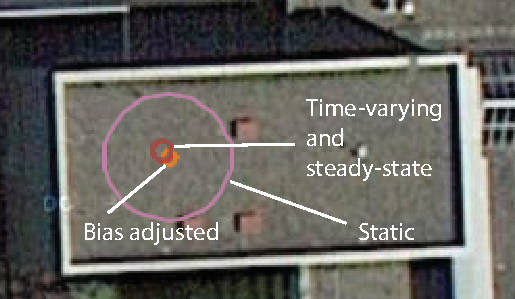
\includegraphics[width=\columnwidth]{stationary_map}
\caption{Static filter results are indicated with a large circle for clarity.  Kalman-filtered results are shown with their 99\% confidence interval ellipses projected onto the East-North plane.}
\label{fig:stationary_map} 
\end{figure}


\subsection{Stationary Receiver}
Figure~\ref{fig:stationary_map} shows the estimated position of the receiver's antenna at the end of the dataset sequence.  The consistency test was used to tune the process covariance matrix to $2\times10^{-3}I$ and the measurement covariance matrix was not rescaled.

Using the antenna's surveyed location, we computed the positional error.  Figure~\ref{fig:stationary_error} shows that during some samples, the bias adjustment model reduces error and it does not severely hinder performance at any sample time.  Our consistency test also passes when bias adjustment is enabled.  While we see some modest improvement for this stationary dataset, we do not observe appreciable benefits on any of the mobile datasets.

\begin{figure}
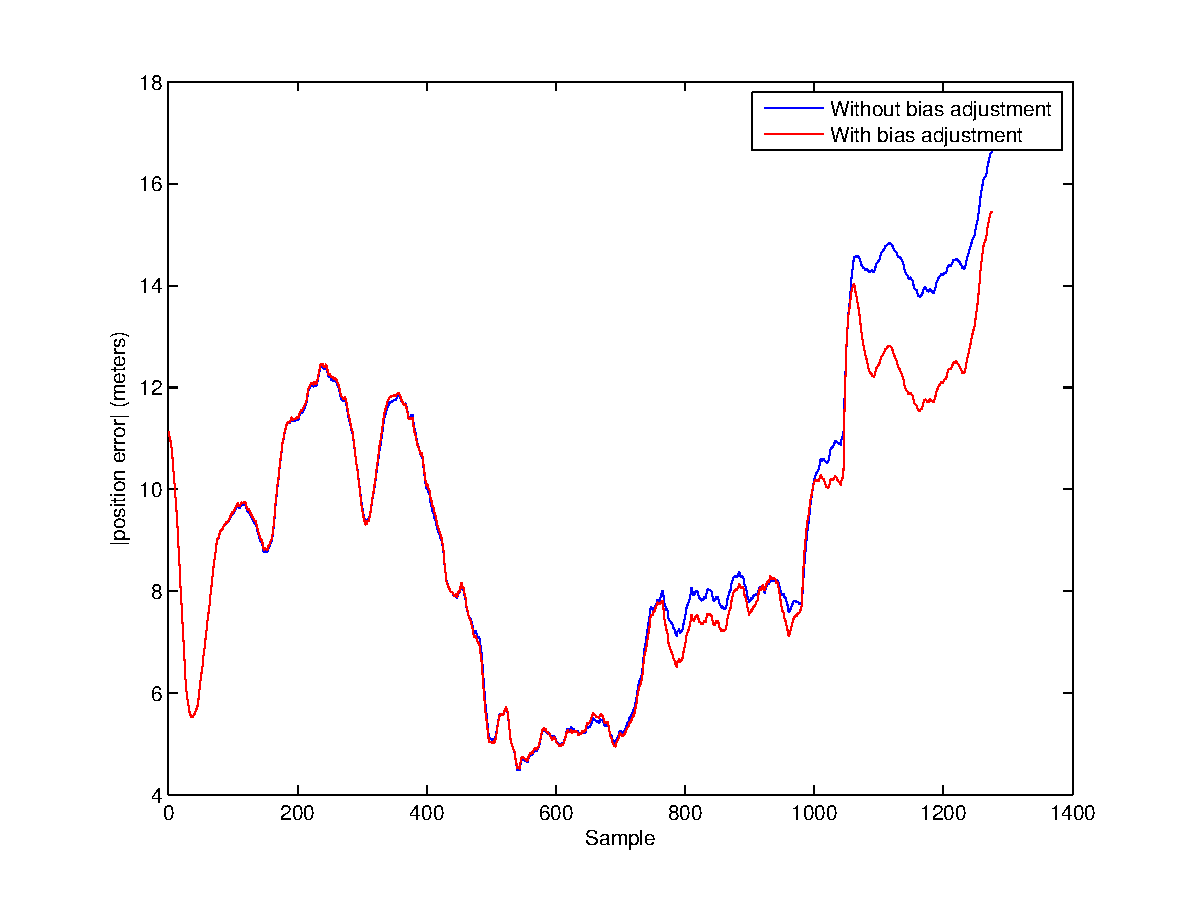
\includegraphics[width=\columnwidth]{error_stationary}
\caption{Error of estimated receiver antenna position with respect to sample time.  The bias adjusted model outperforms the base model in some cases.}
\label{fig:stationary_error}
\end{figure}

Finally, we apply the Ljung-Box test and Mardia's test to the estimated jerk of the system to check for process model mismatch for the case of the time-varying Kalman filter without bias adjustment.  The Ljung-Box test with $\alpha = 0.05$ rejects the null hypothesis test which means the jerk is correlated.  It accepts $H_0$ for Mardia's test with p-value 0.48 for the skewness statistic and 0.1242 for the kurtosis statistic.  When applied to the bias-adjusted version of the time-varying Kalman filter, Mardia's test rejects $H_0$ suggesting that we are indeed introducing a new systematic bias.

Figure~\ref{fig:nis_stationary} shows how the normalized innovation squared statistic, $t_k$ changes over time.  The green lines indicate the test bounds for a 99\% confidence interval and the blue line indicates the test value.  These normalized innovation squared values were fairly consistent, so it seems likely that this is a good way to tune the filter parameters and expect it to generalize well.

\begin{figure}
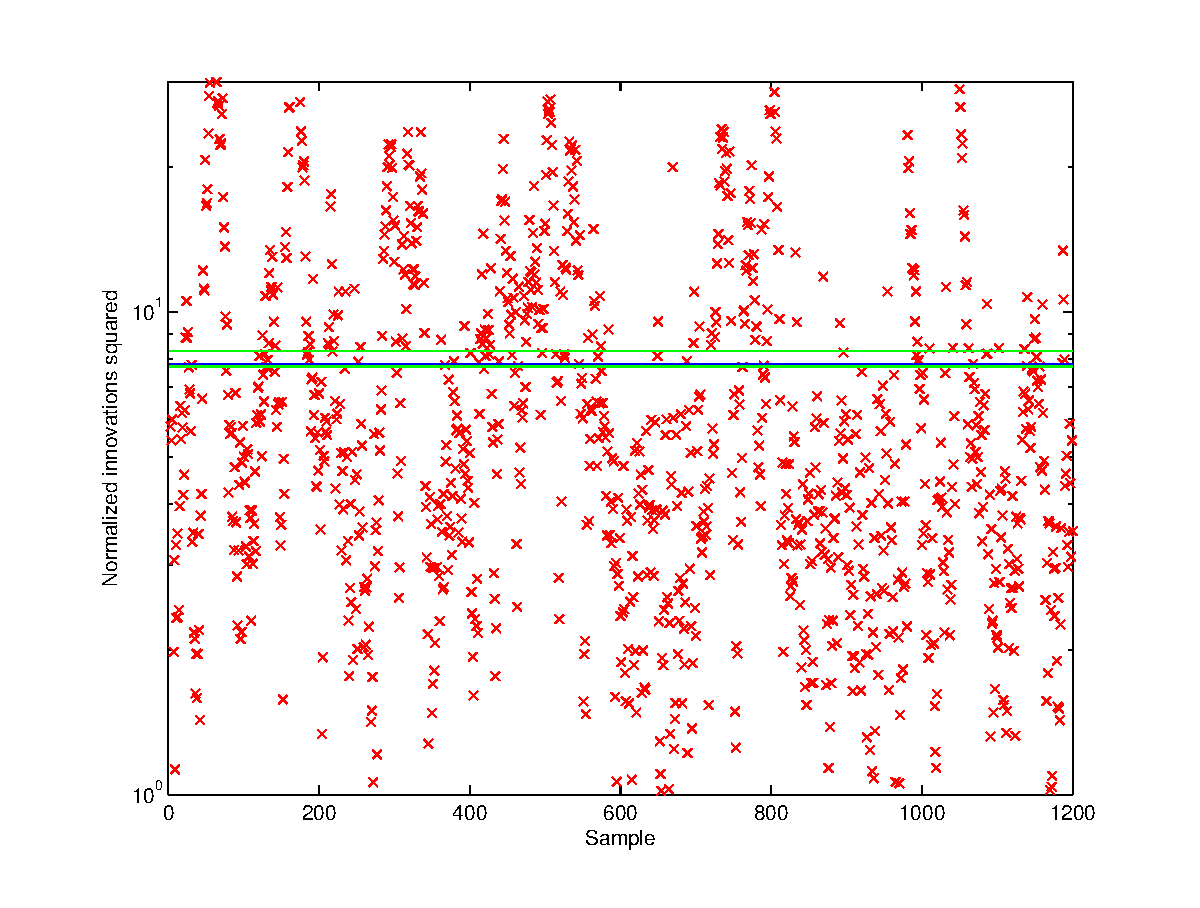
\includegraphics[width=\columnwidth]{nis_stationary}
\caption{Normalized innovation squared values for the \texttt{stationary} dataset.  The green lines represent the test bounds and the blue line is the test statistic.}
\label{fig:nis_stationary}
\end{figure}



\subsection{Airport Dataset}
Figure~\ref{fig:airportloop_map} shows the estimated trajectory of the vehicle using our time-varying Kalman filter.  This was estimated using a process covariance matrix of $Q = 10I$ and a measurement covariance matrix scaled by $3.5$ in order to pass the consistency test.  This is a very easy dataset.  Figure~\ref{fig:airportloop_map_bad} illustrates what happens if we do not scale the measurement covariance matrix to ensure a consistent filter.

\begin{figure}[!bthp]
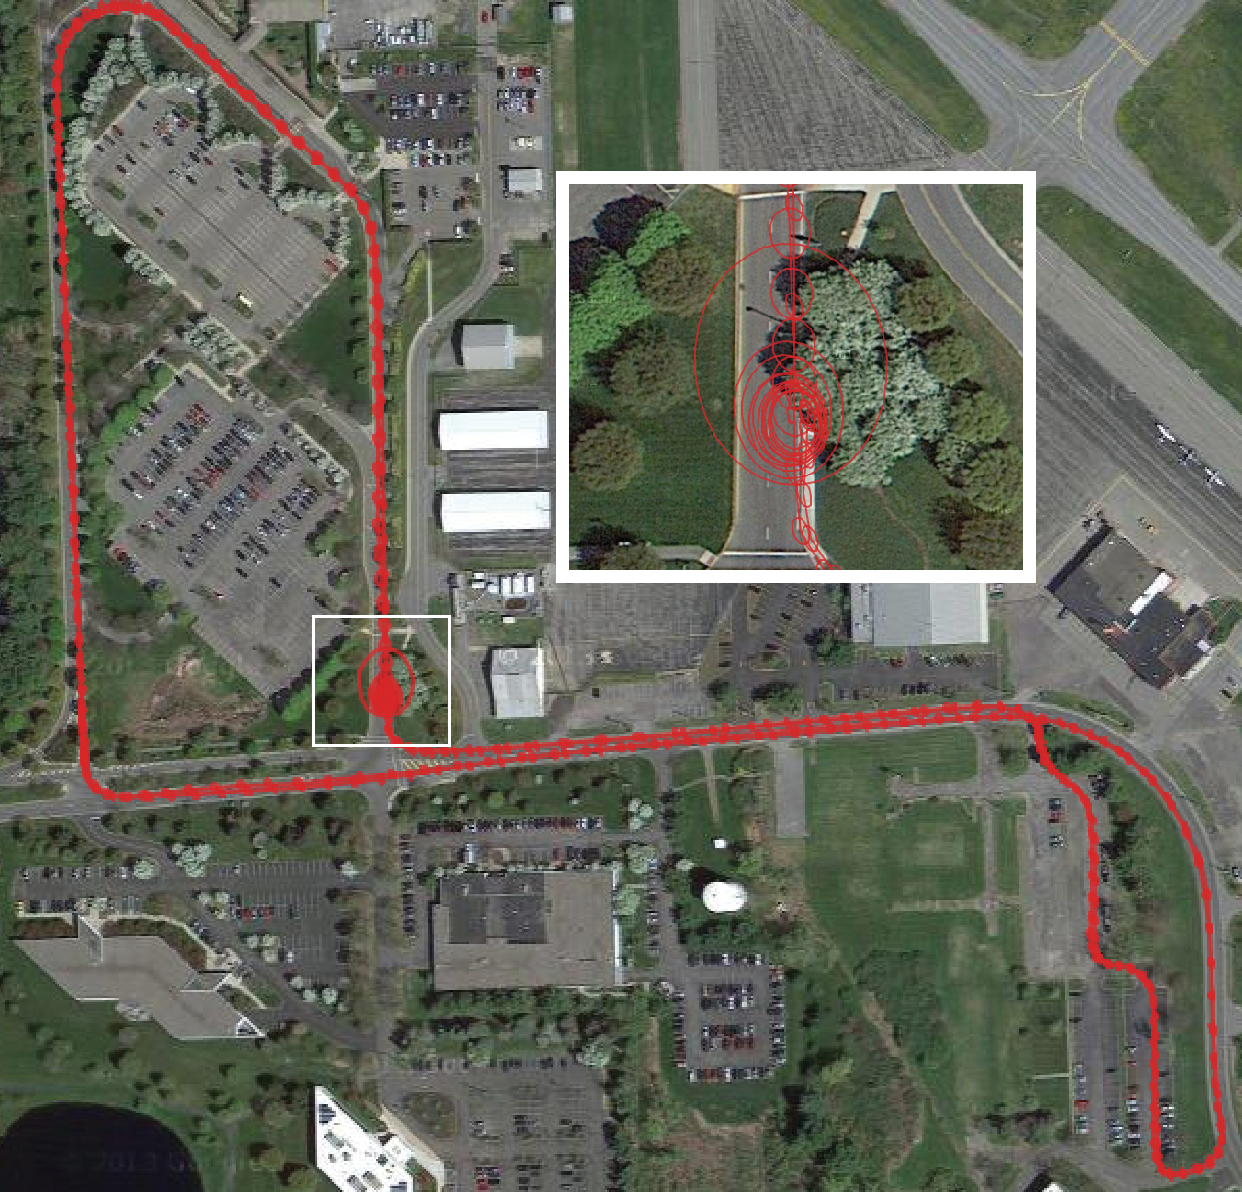
\includegraphics[width=\columnwidth]{airportloop_map}
\caption{Estimated trajectory for \texttt{airportloop} using time-varying Kalman filter adjusted to pass consistency test.  Inset: Initial convergence of estimator at the beginning of the sequence.}
\label{fig:airportloop_map}
\end{figure} 

\begin{figure}
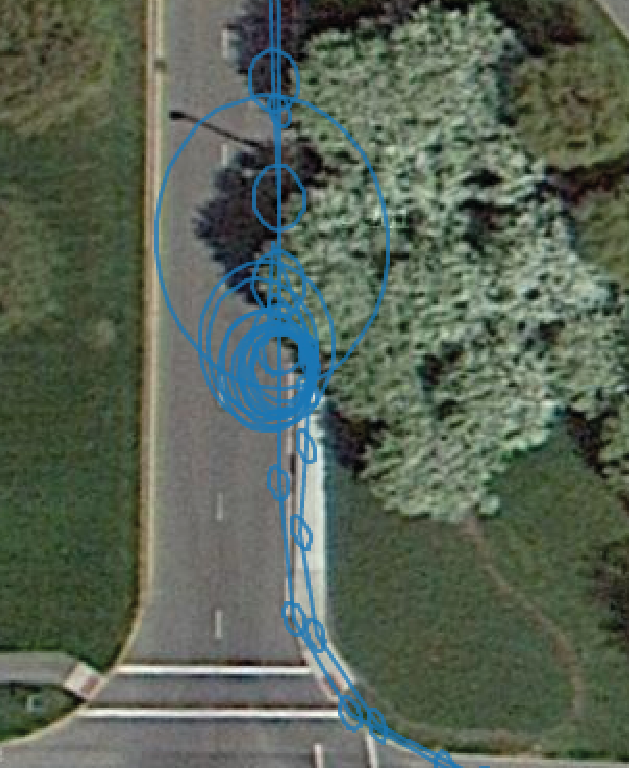
\includegraphics[width=\columnwidth]{airportloop_map_bad}
\caption{Without ensuring filter consistency, the filter can grow over-confident and Kalman filter assumptions that lead to optimality can be broken.  Left: The vehicle is estimated to be on the sidewalk with high confidence.  Right: The original navigation solution is highly erroneous.}
\label{fig:airportloop_map_bad}
\end{figure}

Figure~\ref{fig:nis} shows how the normalized innovations squared statistic, $t_k$ changes over time.  The green lines indicate the test bounds for a 99\% confidence interval and the blue line indicates the test value.  There is a very narrow range for this test to succeed and the trend of the points indicates that even though we successfully found model parameters that helped pass this test, in real world online scenarios, it would be very difficult to do so as subwindows of this data produce different statistics.  This suggestes that our model does not match the system exactly.

\begin{figure}[!b]
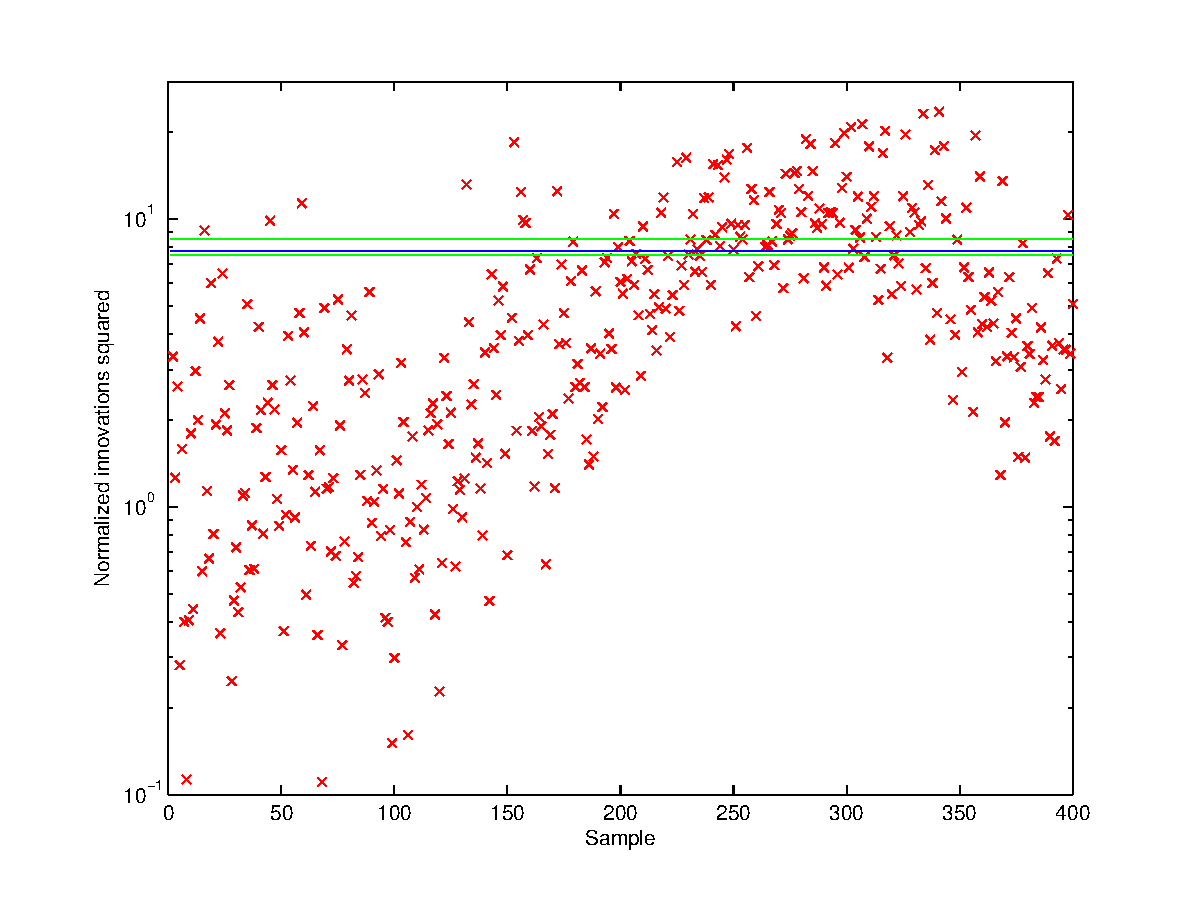
\includegraphics[width=\columnwidth]{nis}
\caption{Normalized innovation squared values for the \texttt{airportloop} dataset.  The green lines represent the test bounds and the blue line is the test statistic.}
\label{fig:nis}
\end{figure}

Since our time-varying Kalman filter propagates an error covariance matrix through the track, we can also evaluate its performance when there is an outage.  Rather than skip missing observations entirely, we perform the prediction step and propagate the a priori state estimate forward.  If we skipped the missing entries entirely, then the estimate's covariance matrix would not adequately grow to accomidate any mismatch between the process and the model.  It also improves the numerical integration of the vehicle's trajectory.  Figure~\ref{fig:outage} shows one such outage.  GPS measurements are disabled for 5 seconds.  The process covariance matrix was tuned down to $Q = 0.1I$ to improve visualization.

\begin{figure}[!t]
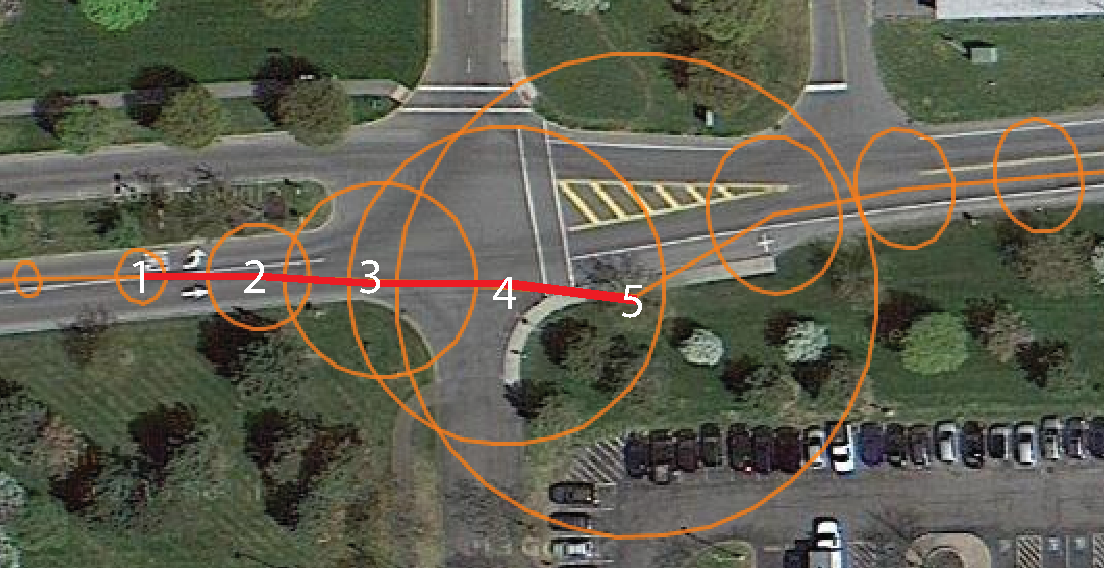
\includegraphics[width=\columnwidth]{outage}
\caption{An artificial 5 second outage during the \texttt{airportloop} dataset.  A priori state estimates during outage marked 1-5.}
\label{fig:outage}
\end{figure}

This dataset did not exhibit any measurements with a large degree of corruption, so we artifically introduced zero-mean Gaussian noise to the pseudorange measurements for satellite 11 for the same 5 second interval as our outage experiment.  If our online consistency hypothesis test can correctly identify erroneous measurements, then the recovery should look exactly like if we did not make those measurements at all.  Figure~\ref{fig:corruption} shows the divergence between the correct trajectory and the measurement-corrupted trajectory.  It also shows the normalized innovation squared measurements exhibit a large increase during this window.  We were unable to find a reliable way to apply the hypothesis test to automatically detect these outliers since the windowed normalized innovation squared statistic varies over time even without measurement corruption.

\begin{figure}[!b]
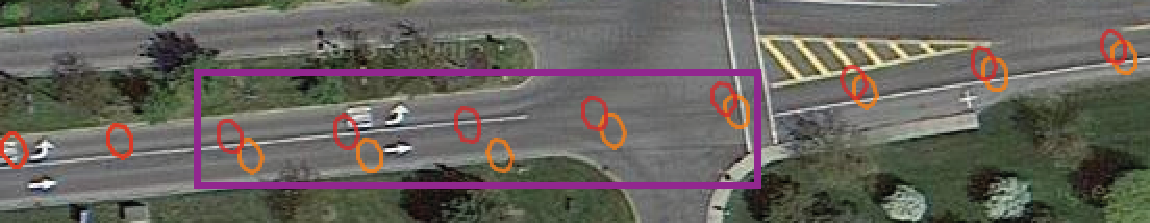
\includegraphics[width=\columnwidth]{corruption}\\
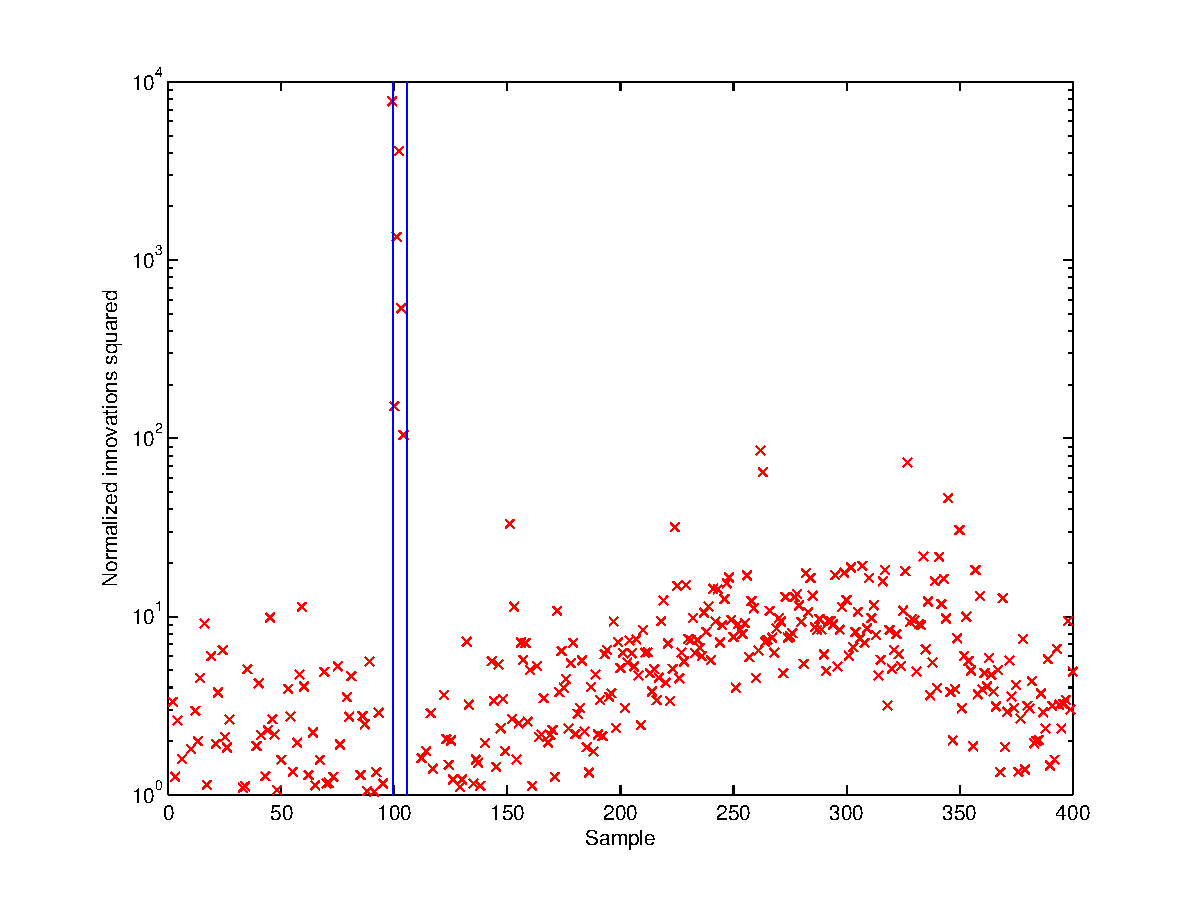
\includegraphics[width=\columnwidth]{nis_corruption}
\caption{Top: Original trajectory in red with corrupted trajectory in orange.  Trajectory is corrupted by introducing zero-mean Gaussian noise to one satellite's pseudorange measurements for 5 seconds, indicated by the violet rectangle.  Bottom: Normalized innovation squared for this sequence.  Blue bars indicate the corruption range.}
\label{fig:corruption}
\end{figure}

\subsection{cudtrt13triphammercu Dataset}
This dataset contains examples of significant drift if velocity is simply integrated.  Figure~\ref{fig:track2_map} shows the different between the time-varying Kalman-filtered track and the integrated track.

\begin{figure}[!b]
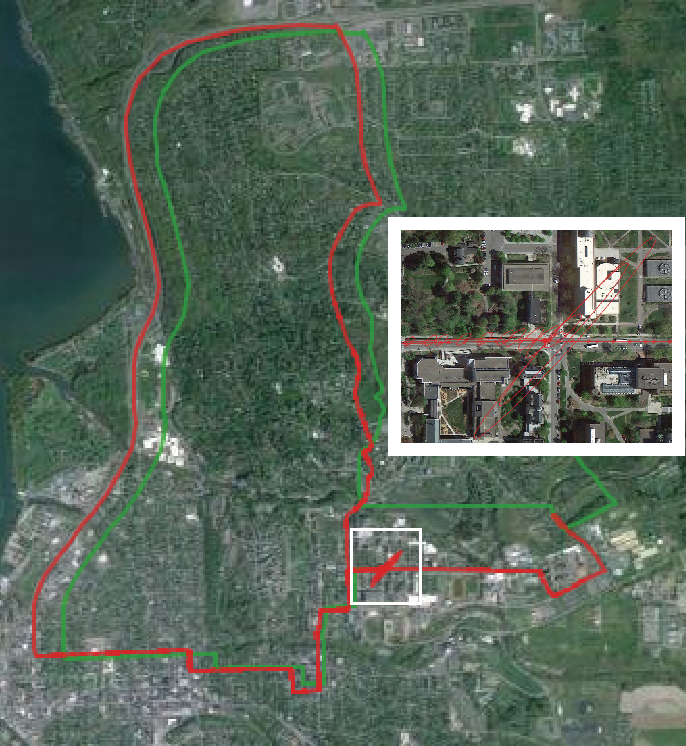
\includegraphics[width=\columnwidth]{track2_map}
\caption{Estimated trajectory for \texttt{cudtrt13triphammercu} dataset using time-varying Kalman filter in red.  Integrated velocity shown in green.  Integrated velocity alone suffers from significant drift.  Inset: Erroneous measurements cause distribution covariance to increase significantly.}
\label{fig:track2_map}
\end{figure}

We artificially introduced the same corruption as for the \texttt{airportloop} dataset, but with a different satellite for 5 seconds on the \texttt{cudtrt13triphammercu}.  The normalized innovation squared values are more consistent in this dataset, so we were able to successfully detect 4 out of 5 corrupt measurements and discard them accordingly.  Figure~\ref{fig:cu_corruption} illustrates how the two trajectories diverge.

\begin{figure}
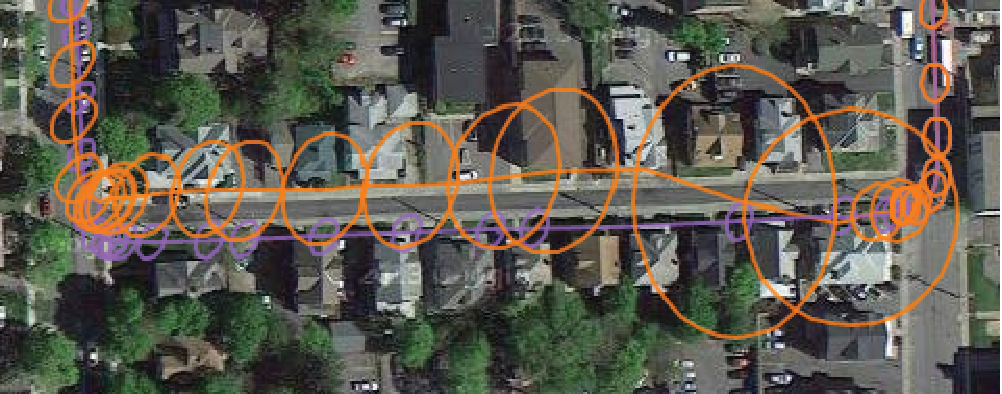
\includegraphics[width=\columnwidth]{cu_corruption}\\
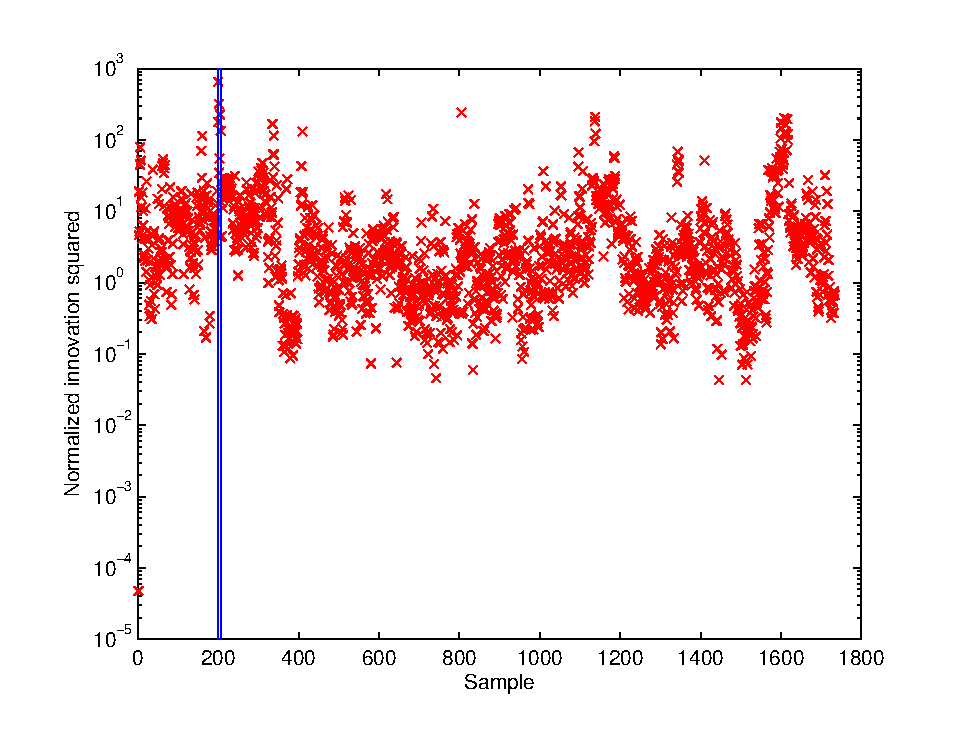
\includegraphics[width=\columnwidth]{nis_cu_corruption}
\caption{Top: The orange estimates are generated by applying the online consistency test to detect faulty measurements while the pink curve becomes biased.  Bottom: The normalized innovation squared values are consistent over time making detection of faulty measurements easy.}
\label{fig:cu_corruption}
\end{figure}

Figure~\ref{fig:max_eigenvalue} shows that for the \texttt{cudtrt13triphammercu} dataset, all eigenvalues are within the unit circle, ensuring a stable filter at each sample time.

\begin{figure}[!t]
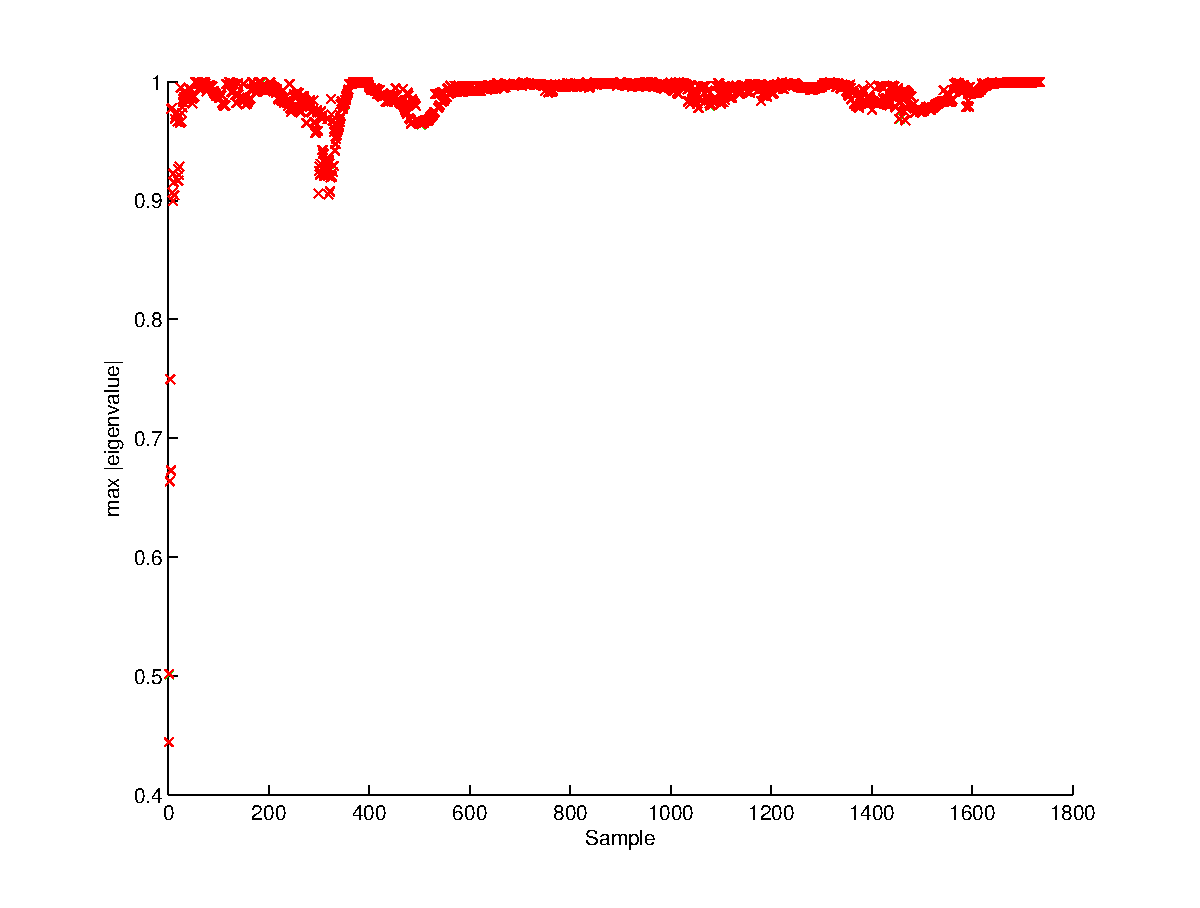
\includegraphics[width=\columnwidth]{eigenvalues}
\caption{Maximum absolute eigenvalues of the closed-loop error dynamics state transition matrix for time-varying Kalman filter on \texttt{cudtrt13triphammercu} dataset.}
\label{fig:max_eigenvalue}
\end{figure}

